\documentclass[11pt,letterpaper]{article}
\usepackage{latex_common/estilo_monitoria}
\usepackage{pdfpages}

\begin{document}

% ============================================================================
% PORTADA GENERAL DEL LIBRO (30 HORAS)
% ============================================================================
\begin{titlepage}
\thispagestyle{empty}
\begin{tcolorbox}[
  enhanced,
  colback=AzulMarino,
  colframe=AzulMarino,
  arc=6pt,
  top=10mm,
  bottom=10mm,
  left=8mm,
  right=8mm,
  boxrule=0pt
]
  \tcbox[on line,colback=Turquesa,colframe=Turquesa,arc=3pt,boxsep=2pt,left=5pt,right=5pt,top=2pt,bottom=2pt]{%
    \footnotesize\sffamily\bfseries\color{white} EDICIÓN COMPLETA DEL CURSO DE MONITORÍA%
  }\hspace{5pt}%
  \tcbox[on line,colback=NaranjaCalido,colframe=NaranjaCalido,arc=3pt,boxsep=2pt,left=5pt,right=5pt,top=2pt,bottom=2pt]{%
    \footnotesize\sffamily\bfseries\color{white} \faClock\hspace{4pt} 30.0 HORAS EXACTAS (15 SESIONES)%
  }\\[14pt]
  {\Huge\bfseries\sffamily\color{white} Algoritmos y Programación\\[4pt] Desde Cero hasta Matrices Estáticas}\\[10pt]
  {\large\sffamily\color{AzulSuave} El viaje paso a paso de \textbf{DFD $\rightarrow$ PSeInt $\rightarrow$ C++ Básico} explicado con plastilina, analogías reales, pruebas de escritorio y simulacros de parcial}
\end{tcolorbox}

\vspace{8mm}
\begin{center}
  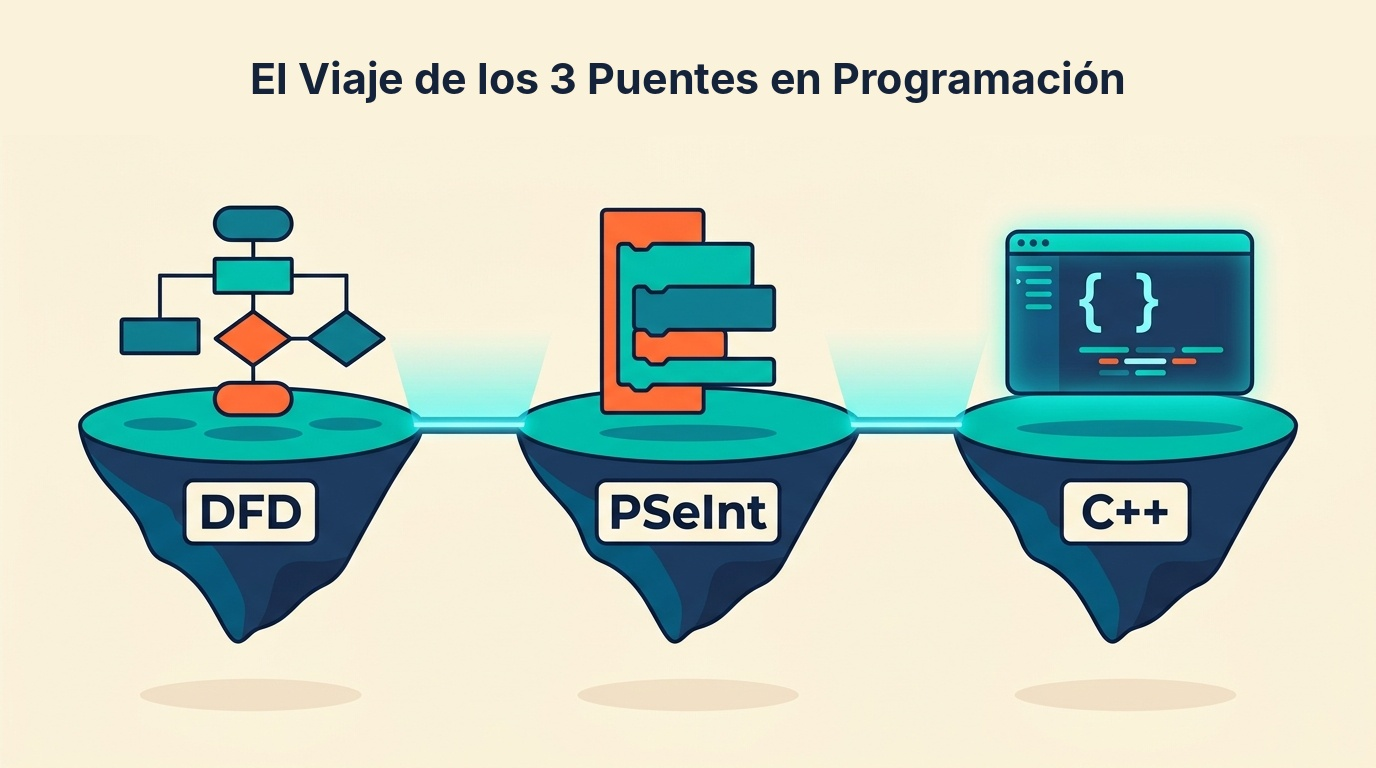
\includegraphics[width=0.88\textwidth]{assets/ilustraciones/ilus_03_puente_dfd_pseint_cpp.jpg}
\end{center}
\vspace{6mm}

\begin{tcolorbox}[
  enhanced,
  colback=TurquesaClaro,
  colframe=Turquesa,
  leftrule=4pt,
  boxrule=0.8pt,
  arc=4pt,
  top=4mm,
  bottom=4mm,
  left=5mm,
  right=5mm,
  title={\faCompass\hspace{0.5em}\textbf{Alcance Técnico Garantizado (Primer Semestre Universitario)}},
  coltitle=white,
  colbacktitle=Turquesa
]
\small
Este libro reúne los \textbf{9 módulos progresivos (M00--M08)} y las \textbf{4 fichas imprimibles} del programa completo de 30 horas. Todo el código en C++ ha sido compilado con \codigo{g++ -std=c++17} usando exclusivamente variables simples, condicionales, ciclos, funciones básicas y \textbf{vectores y matrices estáticos con tamaño fijo definido} (\codigo{const int MAX}), \textbf{sin punteros, sin memoria dinámica ni \texttt{std::vector}}.
\end{tcolorbox}

\vfill
\begin{center}
  {\small\sffamily\color{ComentarioCodigo} Compendio Oficial de Monitoría Académica $\bullet$ Módulos M00--M08 + Fichas Resumen 01--04}
\end{center}
\end{titlepage}

% ============================================================================
% MAPA CURRICULAR DE 30 HORAS Y TABLA DE CONTENIDOS
% ============================================================================
\newpage
\thispagestyle{plain}
\section*{Mapa Curricular del Curso Completo (30.0 Horas)}

\begin{center}
  \small
  \renewcommand{\arraystretch}{1.22}
  \rowcolors{2}{GrisSuave}{white}
  \begin{tabularx}{\textwidth}{>{\bfseries\sffamily\color{AzulMarino}}c >{\raggedright\arraybackslash}X >{\raggedright\arraybackslash}p{5.1cm} >{\bfseries\color{Turquesa}}c}
    \rowcolor{AzulMarino}
    \textcolor{white}{\textbf{Módulo}} & \textcolor{white}{\textbf{Título}} & \textcolor{white}{\textbf{Enfoque central}} & \textcolor{white}{\textbf{Horas}} \\
    \midrule
    M00 & Algoritmos para Tontos & Pensar antes de teclar, EPS, Método 5 Pasos & 2.5 h \\
    M01 & Lógica y Diagramas de Flujo (DFD) & Símbolos oficiales, decisiones, prueba de escritorio & 3.0 h \\
    M02 & PSeInt y el Puente hacia C++ & Pseudocódigo en español, primer programa C++ & 3.0 h \\
    M03 & Tipos de Datos, RAM y Operadores & \texttt{int}, \texttt{double}, \texttt{char}, \texttt{bool}, \texttt{string}, \texttt{/}, \texttt{\%}, casting & 3.0 h \\
    M04 & Estructuras Condicionales & Lógica booleana, \texttt{if-else}, \texttt{else-if}, \texttt{switch} & 3.5 h \\
    M05 & Ciclos y Bucles & \texttt{for}, \texttt{while}, \texttt{do-while}, centinelas, anidados & 4.0 h \\
    M06 & Vectores Estáticos (1D) & Capacidad fija \texttt{MAX}, búsqueda, inserción, Burbuja & 4.0 h \\
    M07 & Matrices Estáticas (2D) & Filas vs. columnas, diagonales, simetría, casos reales & 4.0 h \\
    M08 & Modularidad y Simulacros de Parcial & Funciones, valor vs. \texttt{\&}, estrategia anti-pánico, 2 parciales & 3.0 h \\
    \midrule
    \multicolumn{3}{r}{\textbf{\sffamily TOTAL DEL PROGRAMA COMPLETO DE MONITORÍA}} & \textbf{30.0 h} \\
    \bottomrule
  \end{tabularx}
\end{center}

\vspace{4mm}
\begin{consejo}{Material Complementario Incluido al Final del Libro}
Además de los 9 módulos completos, el apéndice final anexa las \textbf{4 Fichas Resumen Imprimibles} (Símbolos DFD, Traductor Maestro DFD--PSeInt--C++, Método de los 5 Pasos y Patrones de Vectores y Matrices Estáticos), listas para imprimir en hoja tamaño carta como guía de estudio.
\end{consejo}

\newpage
\thispagestyle{plain}
\tableofcontents

% ============================================================================
% INCLUSION DE MODULOS M00..M08
% ============================================================================
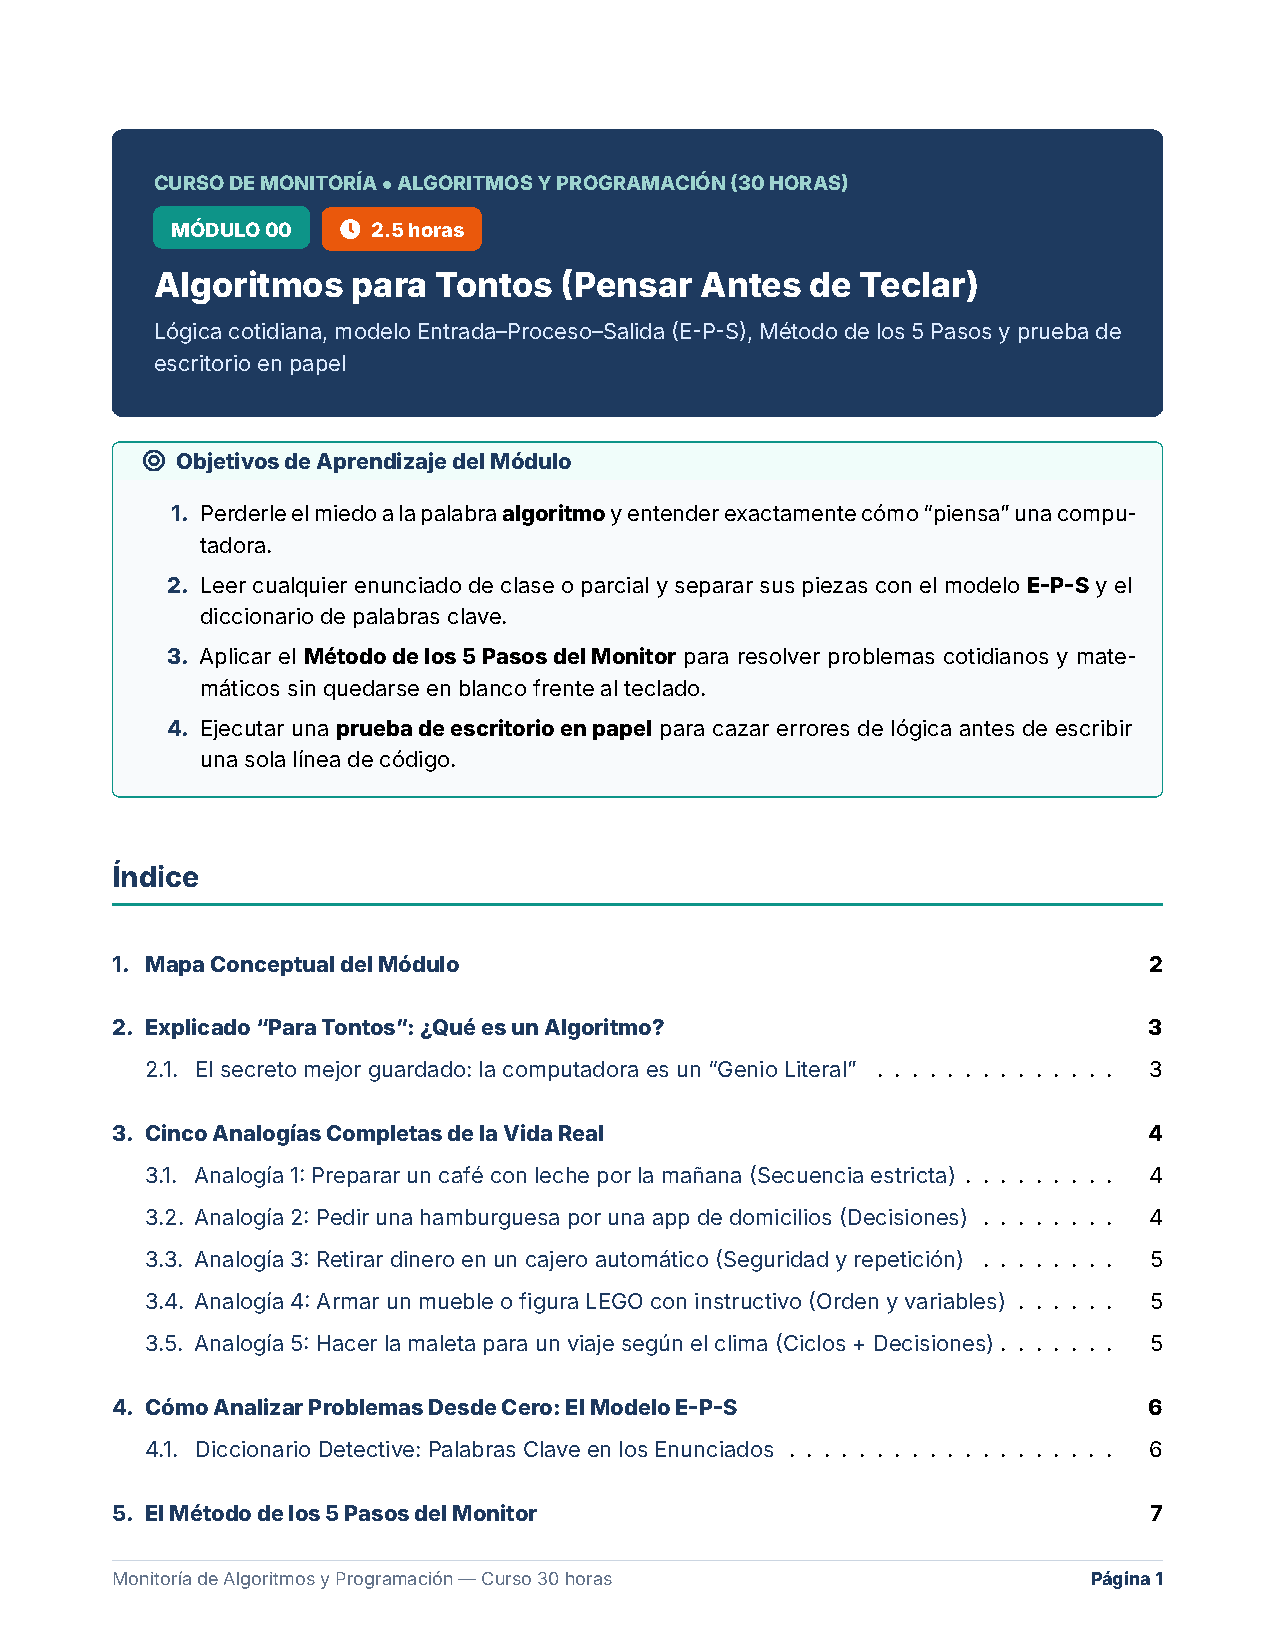
\includepdf[pages=-,addtotoc={1,section,1,{Módulo 00: Algoritmos para Tontos (2.5 h)},m00}]{modulos/M00_Algoritmos_Para_Tontos/M00_Algoritmos_Para_Tontos.pdf}
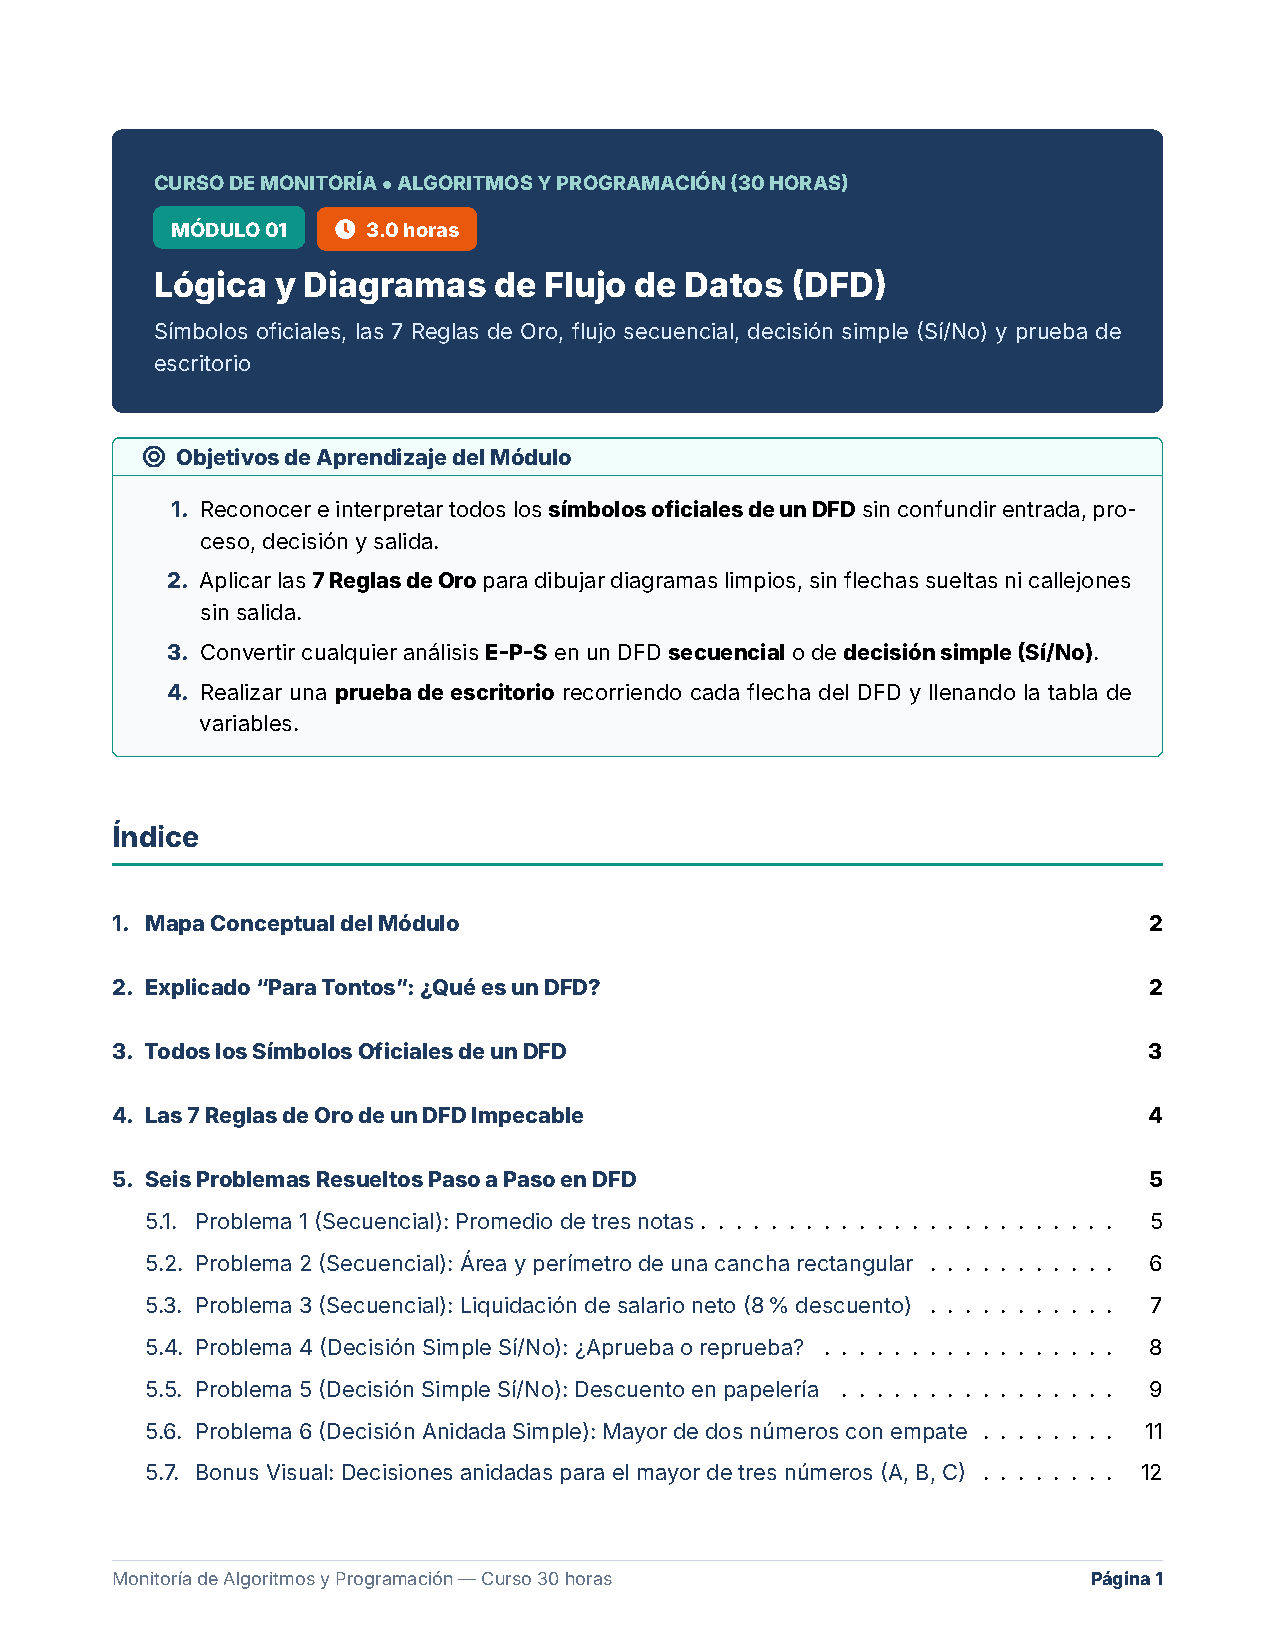
\includepdf[pages=-,addtotoc={1,section,1,{Módulo 01: Lógica y Diagramas de Flujo DFD (3.0 h)},m01}]{modulos/M01_Logica_y_DFD/M01_Logica_y_DFD.pdf}
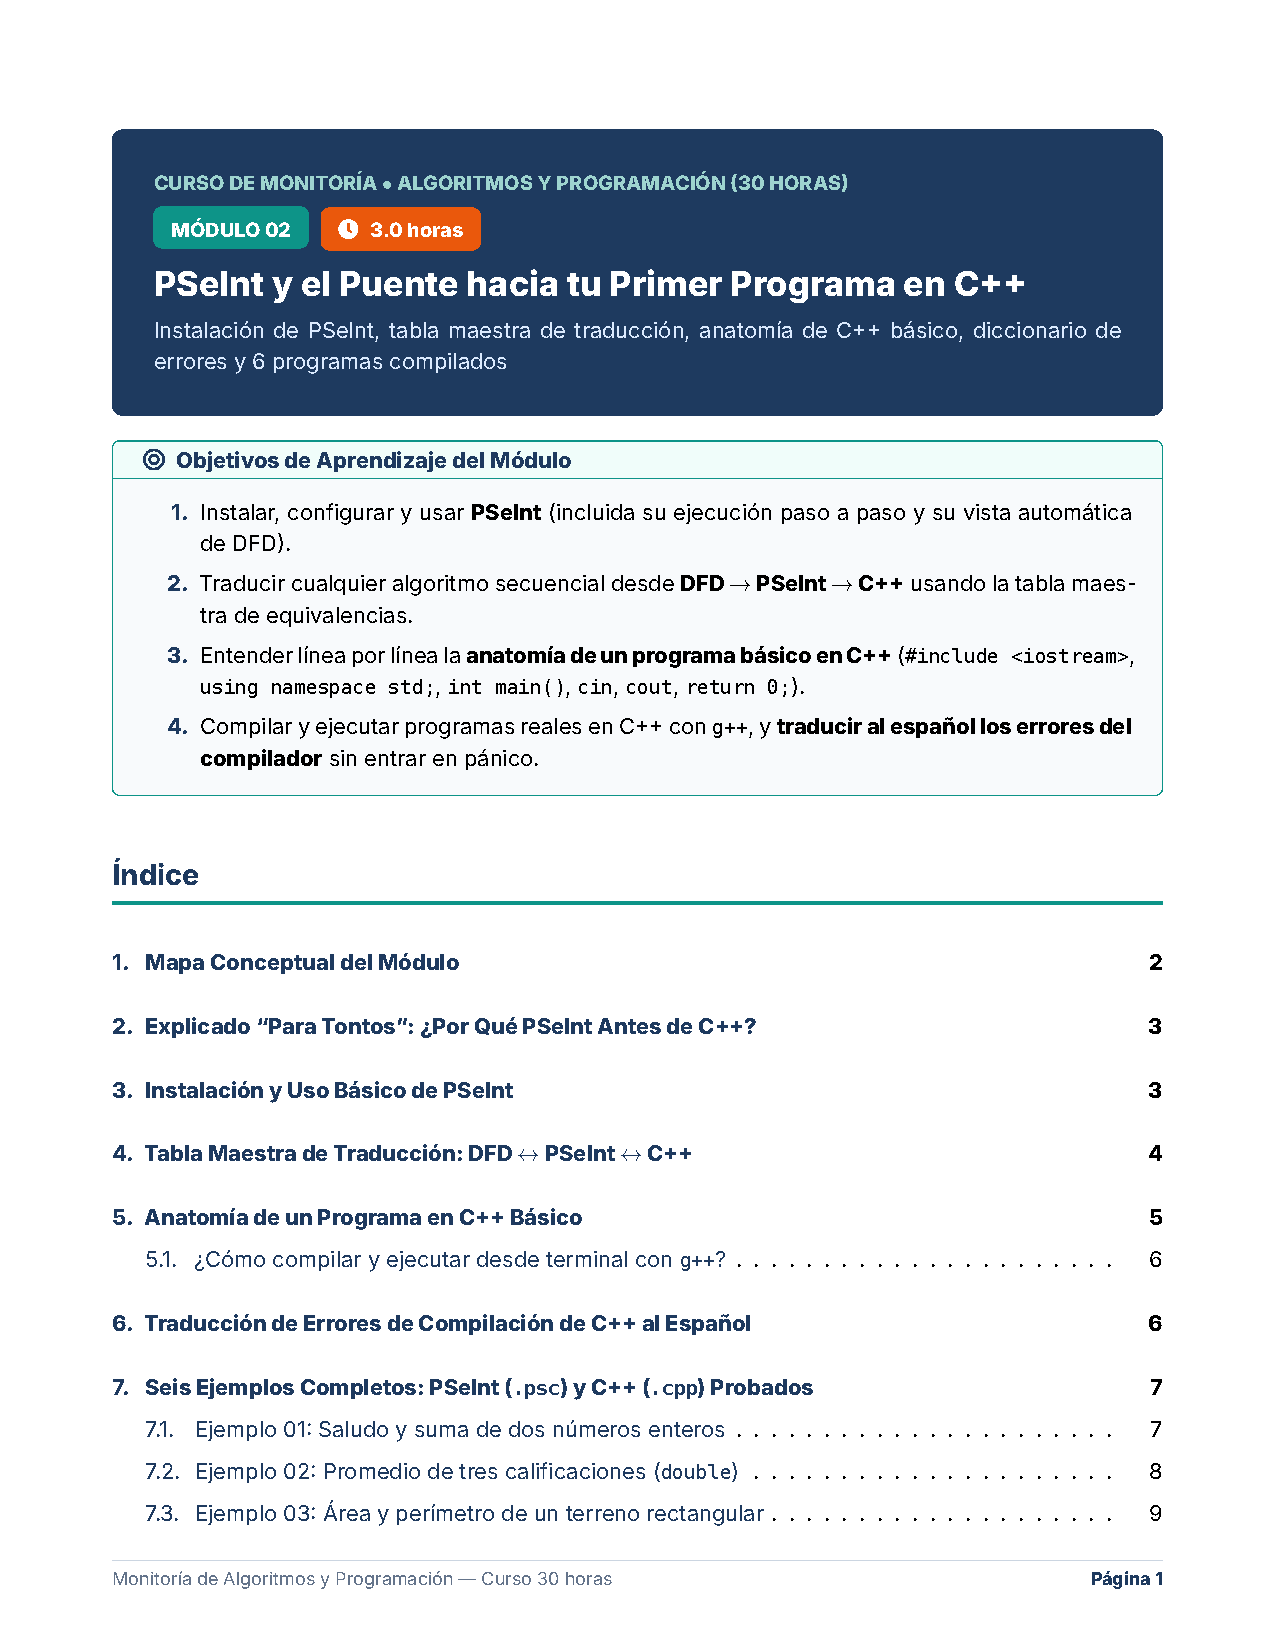
\includepdf[pages=-,addtotoc={1,section,1,{Módulo 02: PSeInt y el Puente hacia C++ (3.0 h)},m02}]{modulos/M02_PSeInt_y_Puente_CPP/M02_PSeInt_y_Puente_CPP.pdf}
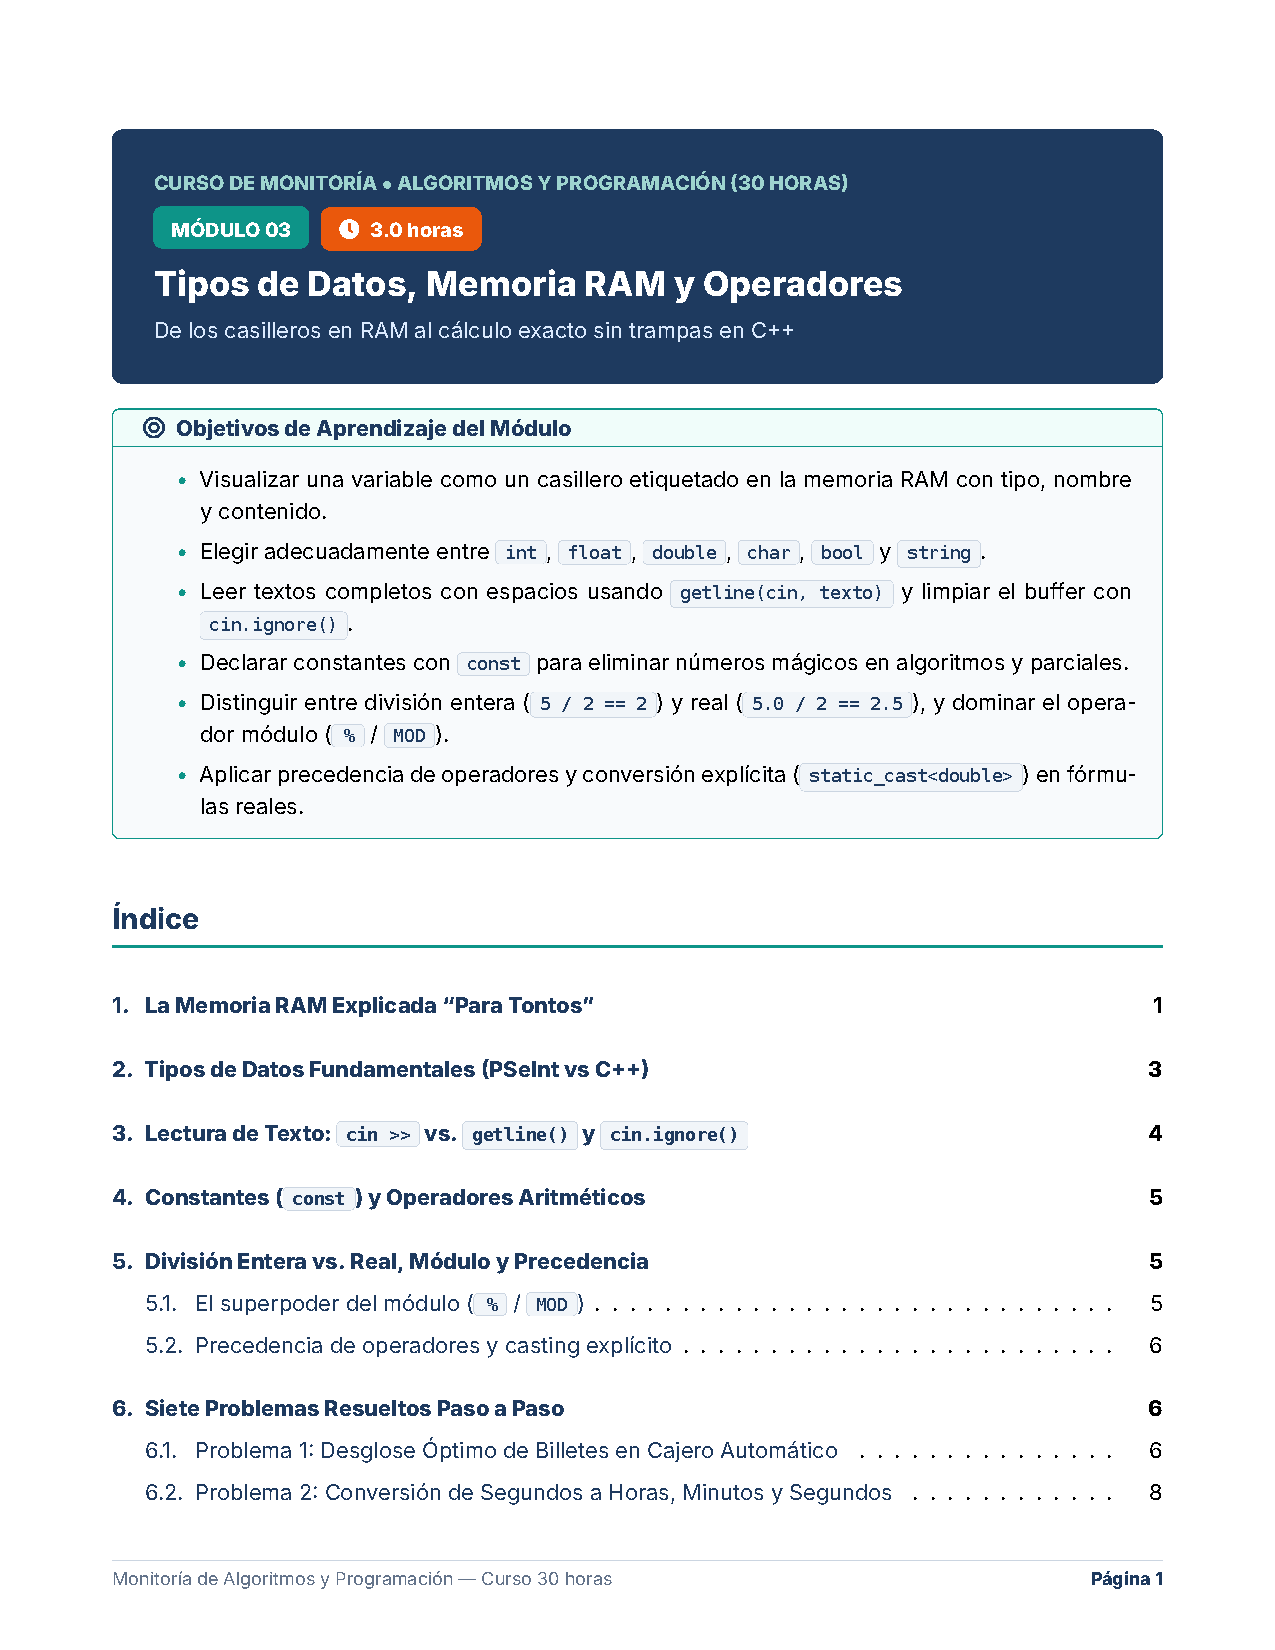
\includepdf[pages=-,addtotoc={1,section,1,{Módulo 03: Tipos de Datos y Operadores (3.0 h)},m03}]{modulos/M03_Tipos_Datos_y_Operadores/M03_Tipos_Datos_y_Operadores.pdf}
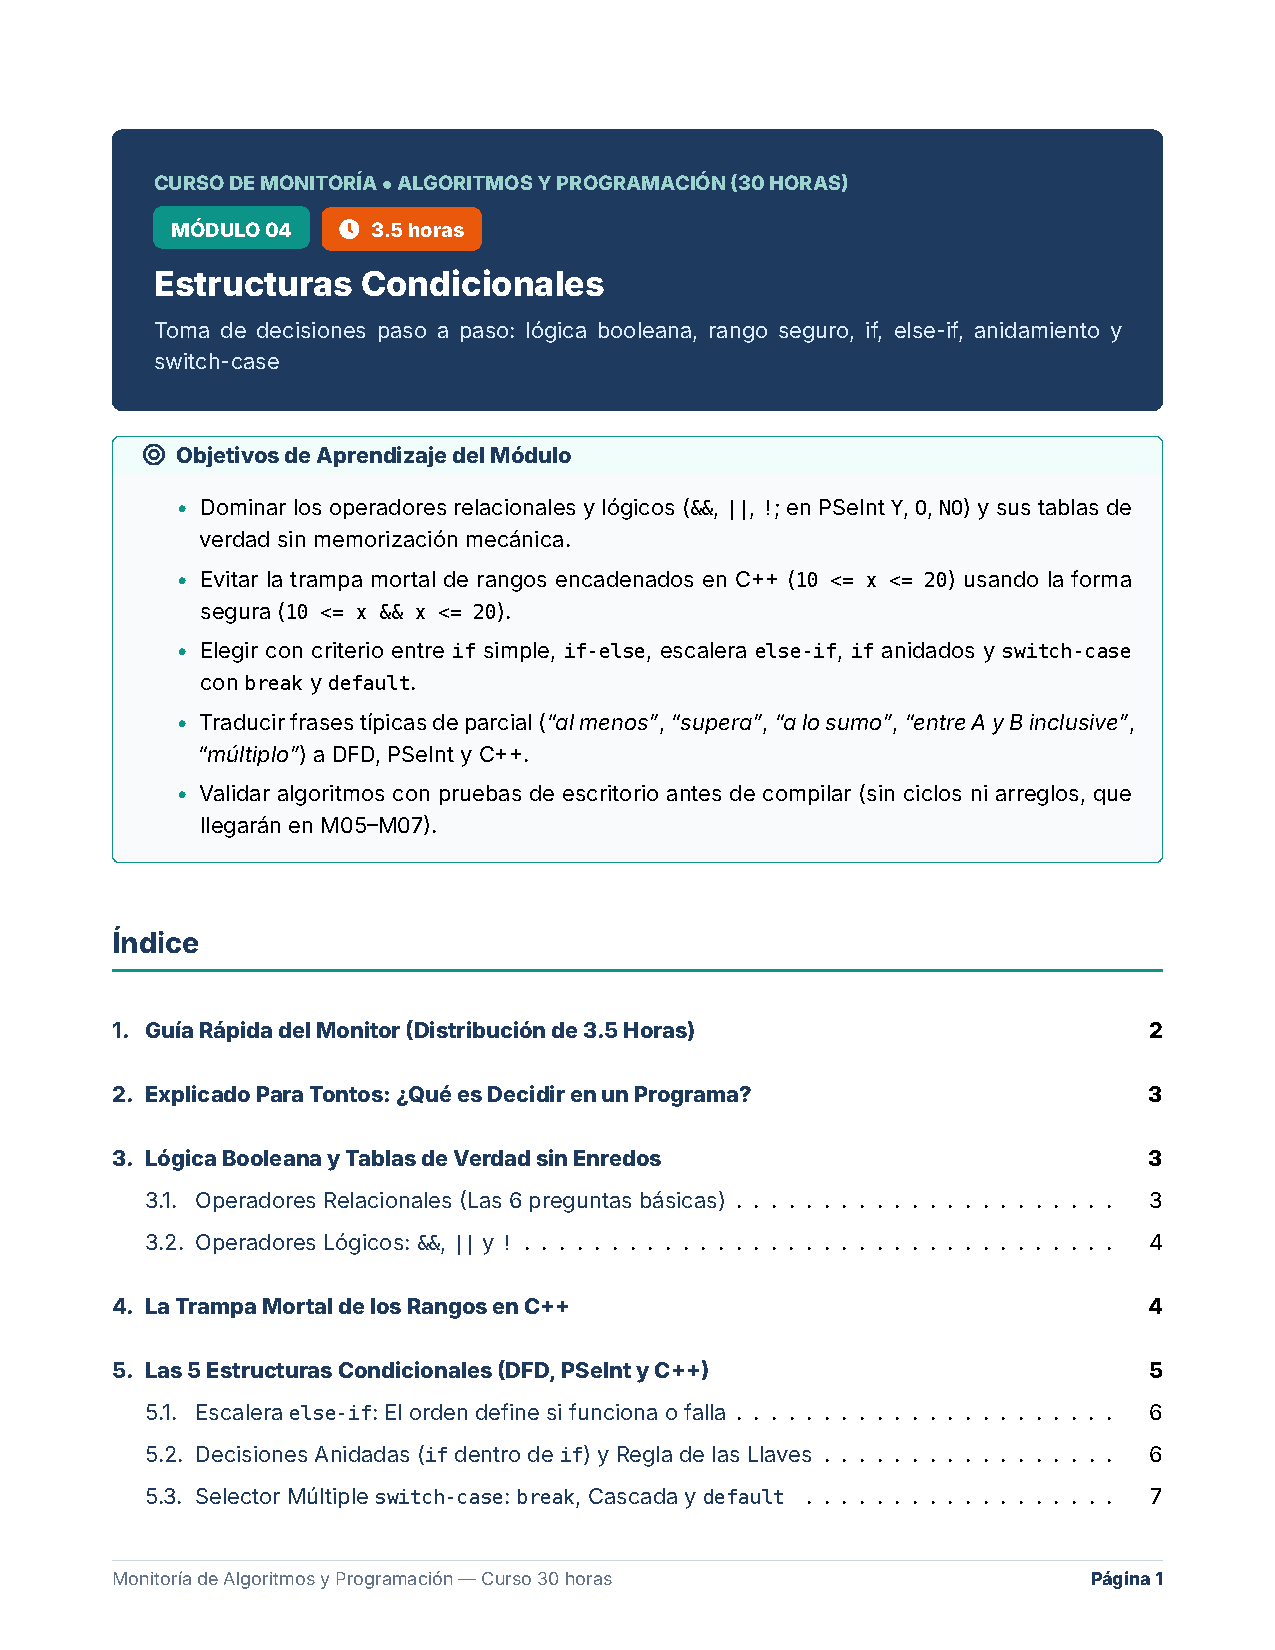
\includepdf[pages=-,addtotoc={1,section,1,{Módulo 04: Estructuras Condicionales (3.5 h)},m04}]{modulos/M04_Condicionales/M04_Condicionales.pdf}
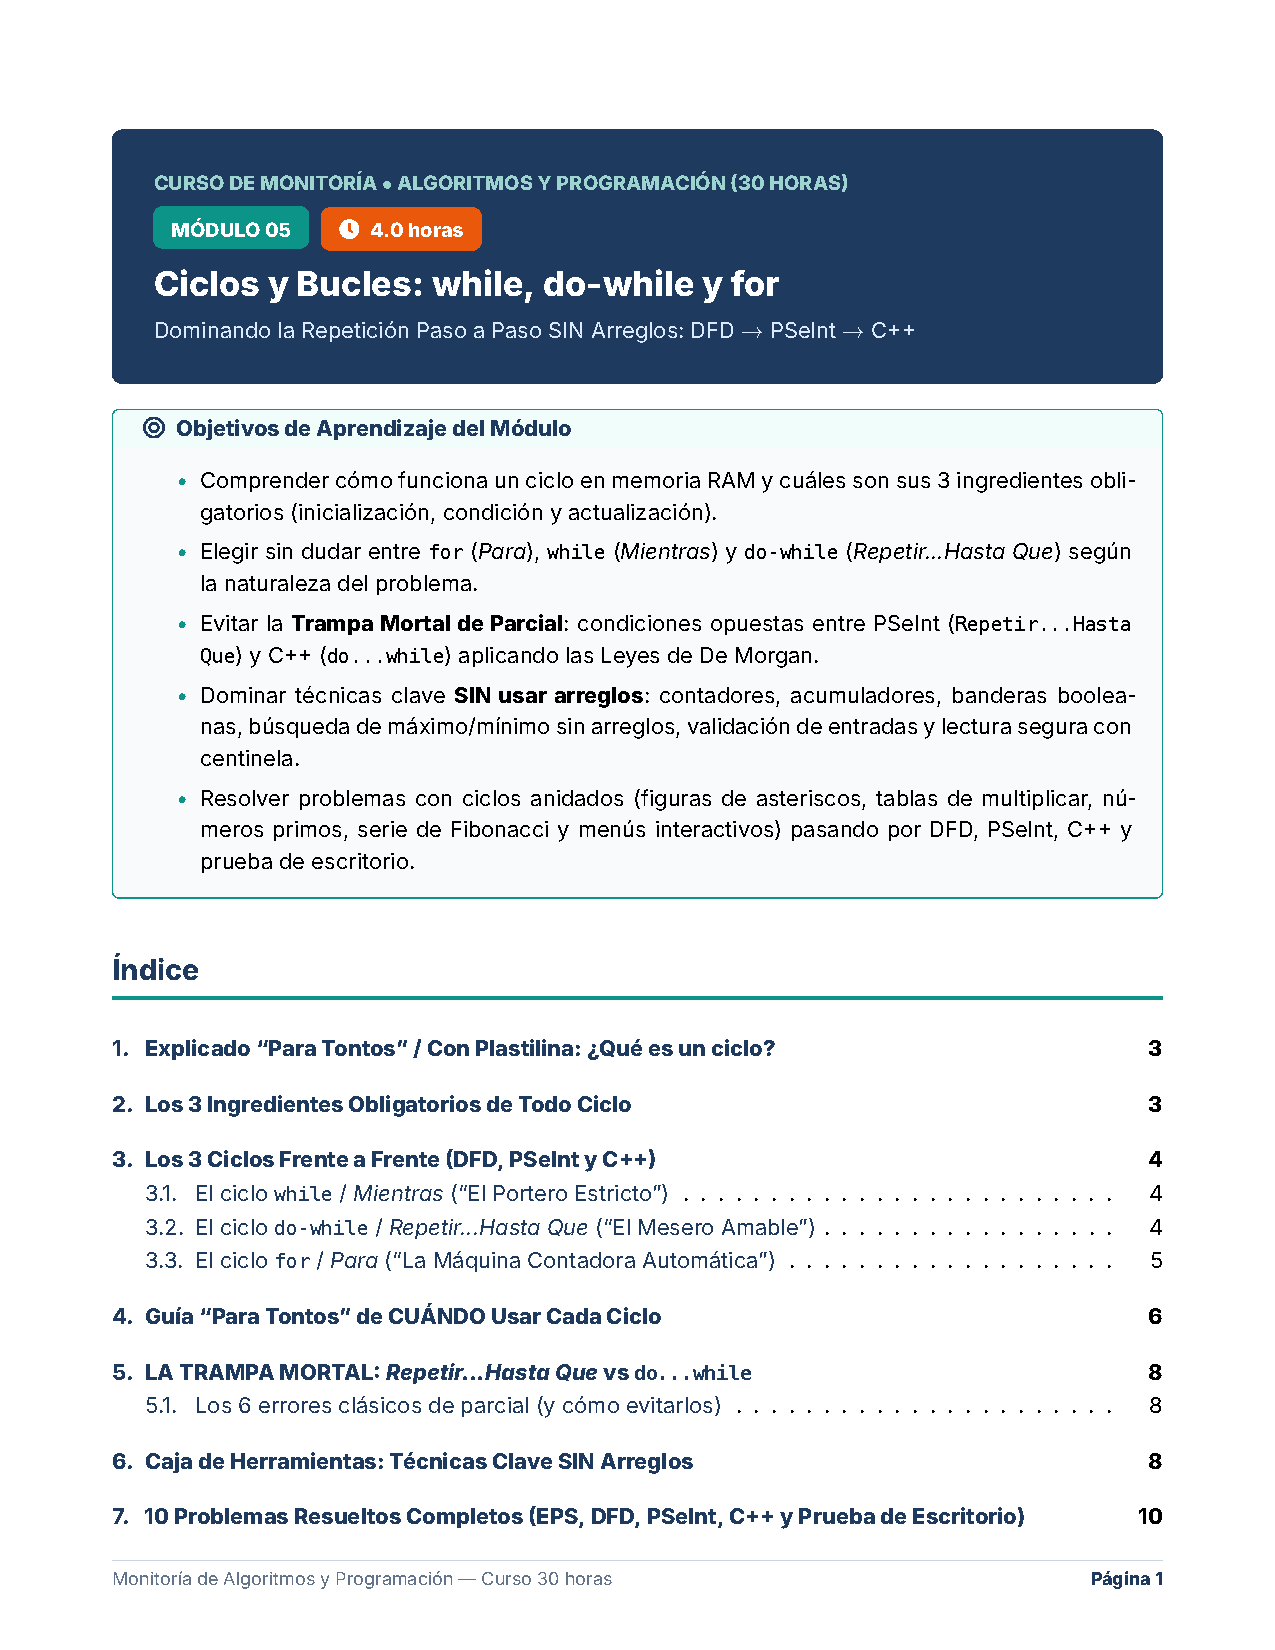
\includepdf[pages=-,addtotoc={1,section,1,{Módulo 05: Ciclos y Bucles (4.0 h)},m05}]{modulos/M05_Ciclos_y_Bucles/M05_Ciclos_y_Bucles.pdf}
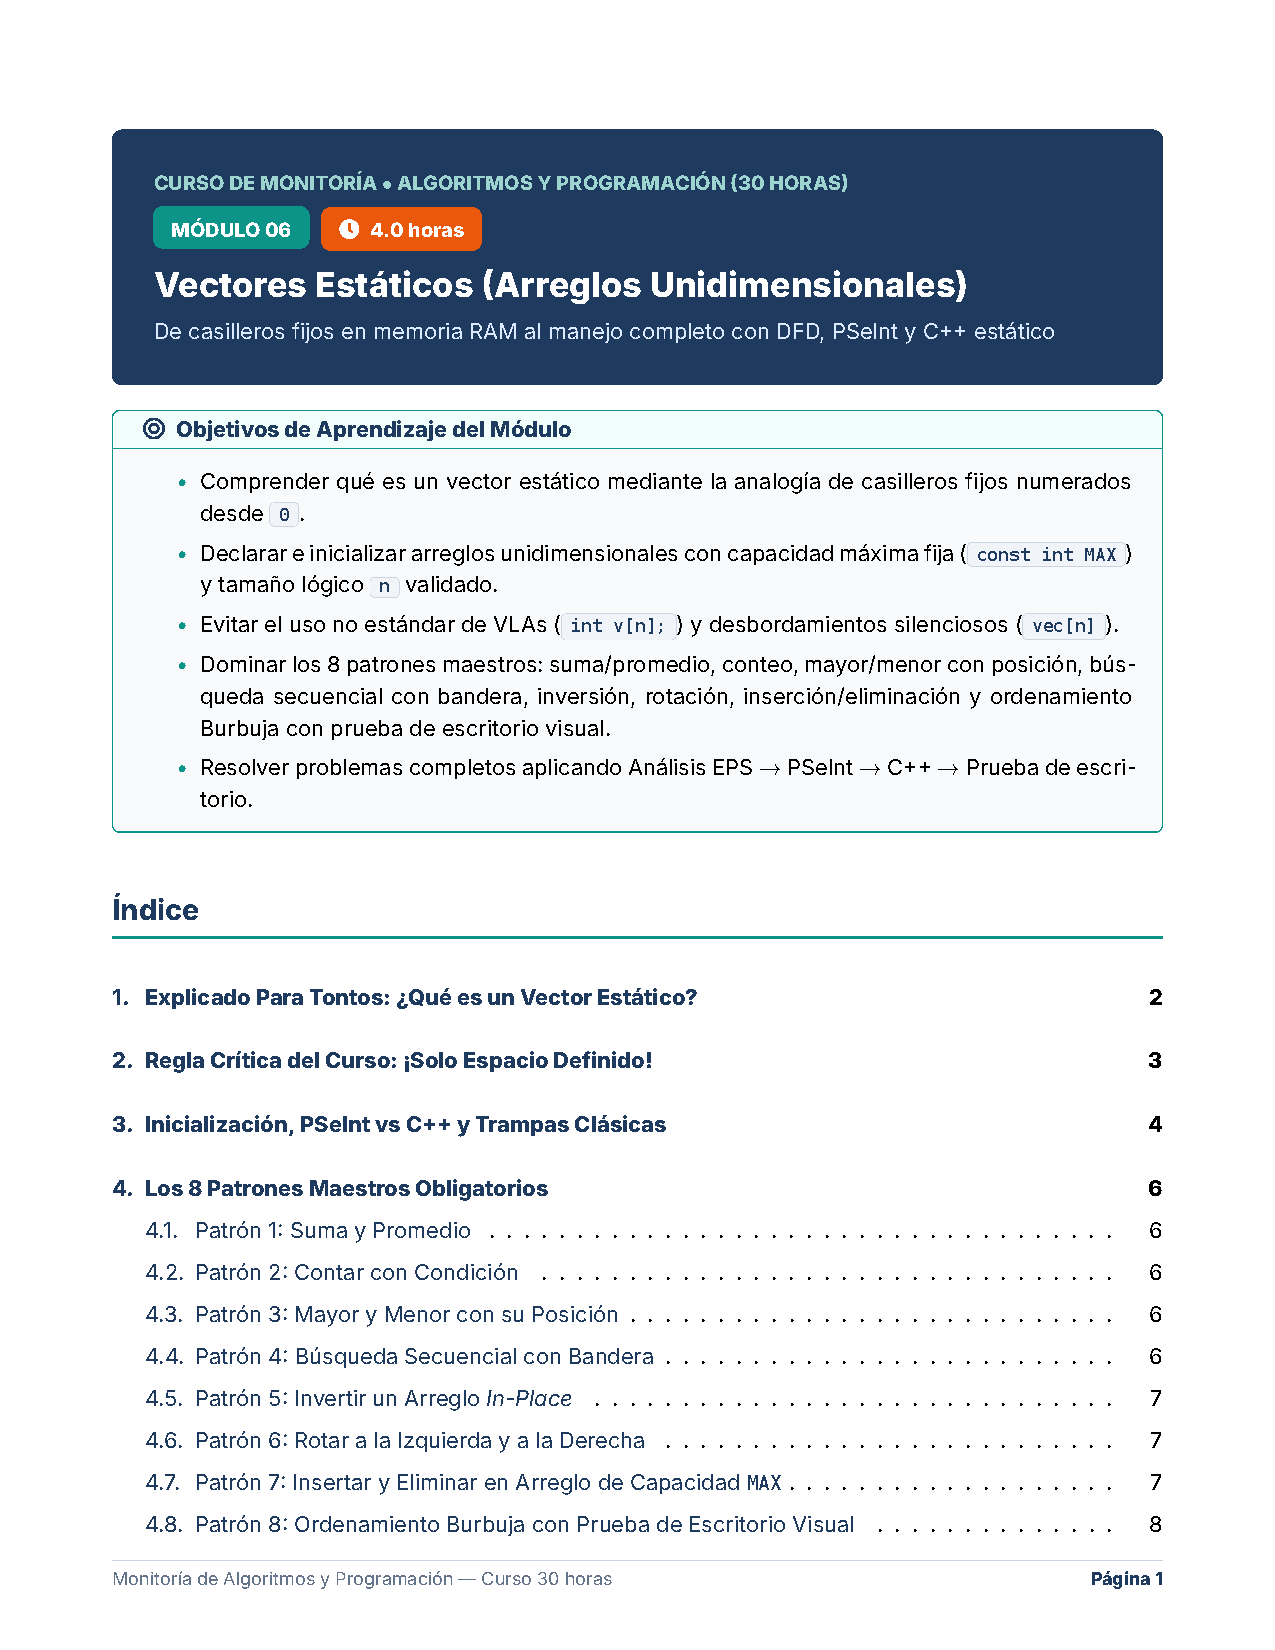
\includepdf[pages=-,addtotoc={1,section,1,{Módulo 06: Vectores Estáticos (4.0 h)},m06}]{modulos/M06_Vectores_Estaticos/M06_Vectores_Estaticos.pdf}
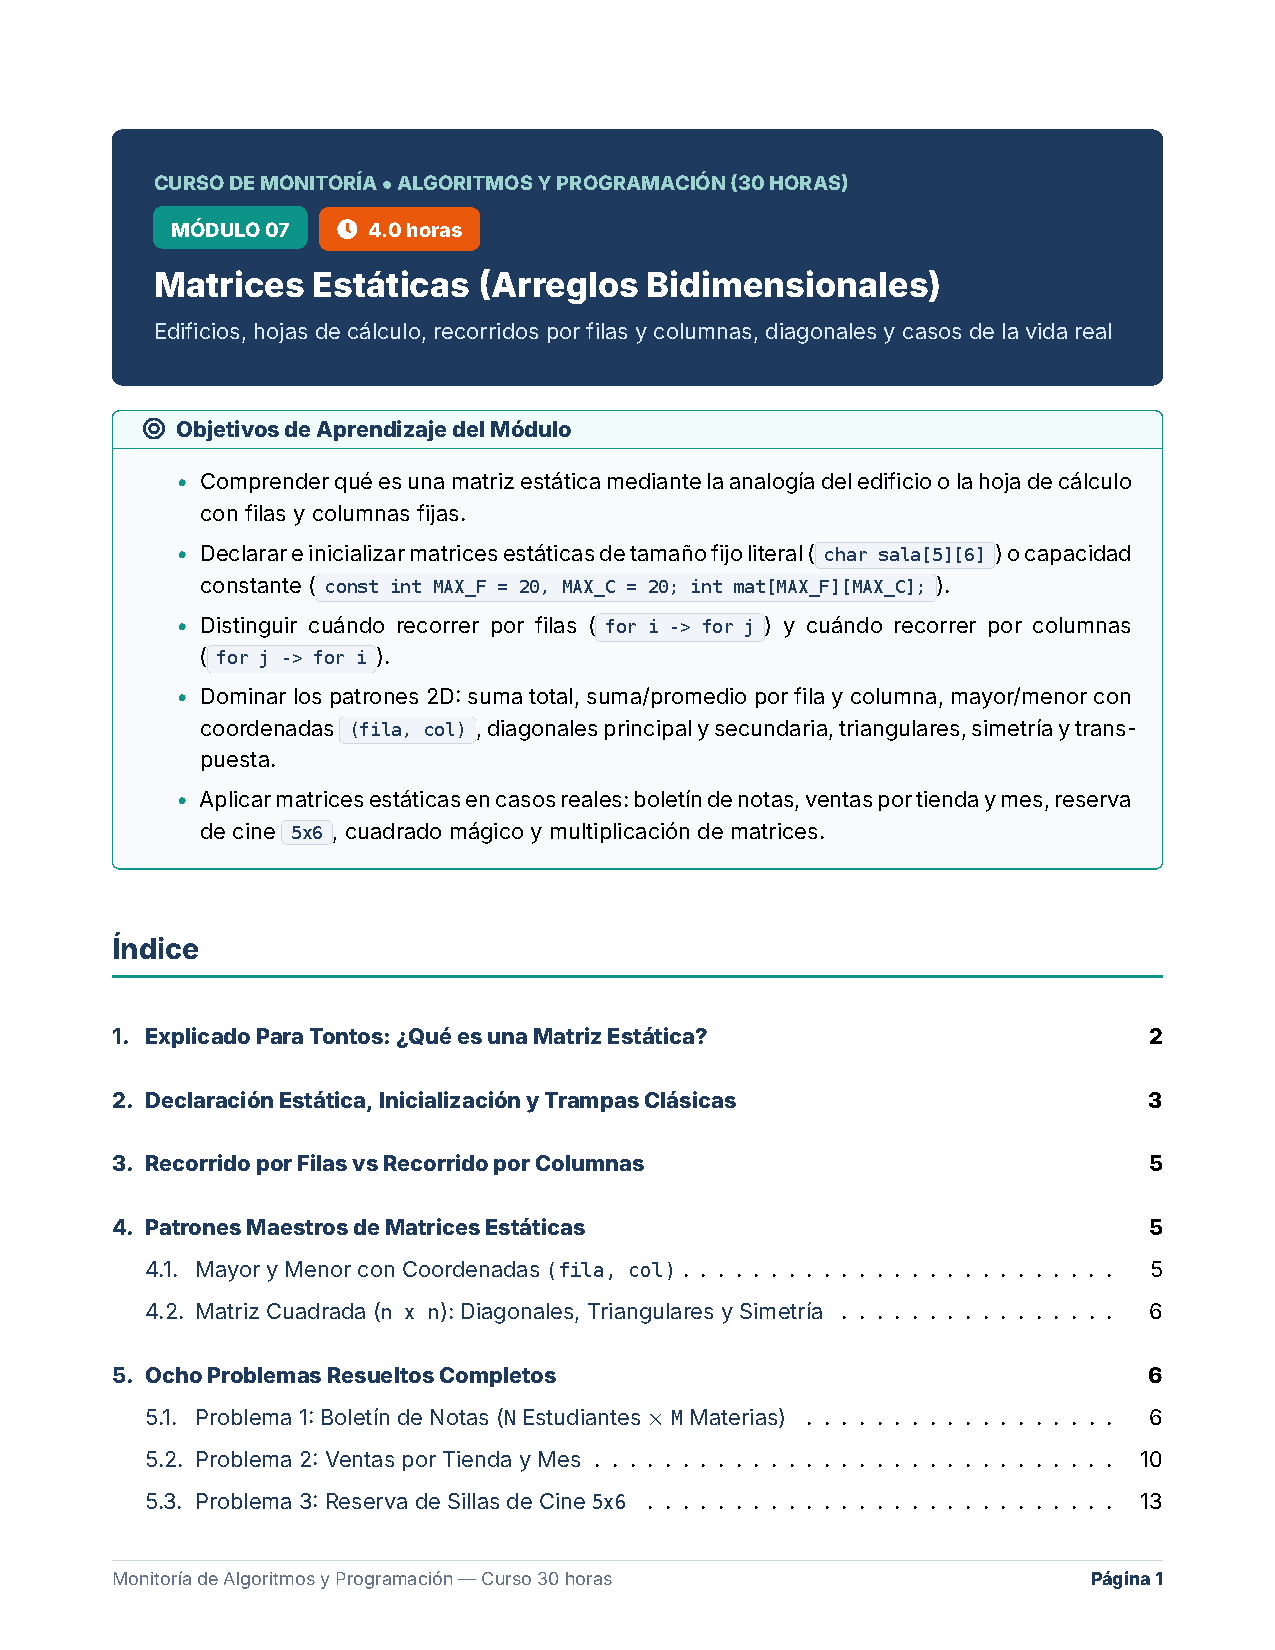
\includepdf[pages=-,addtotoc={1,section,1,{Módulo 07: Matrices Estáticas (4.0 h)},m07}]{modulos/M07_Matrices_Estaticas/M07_Matrices_Estaticas.pdf}
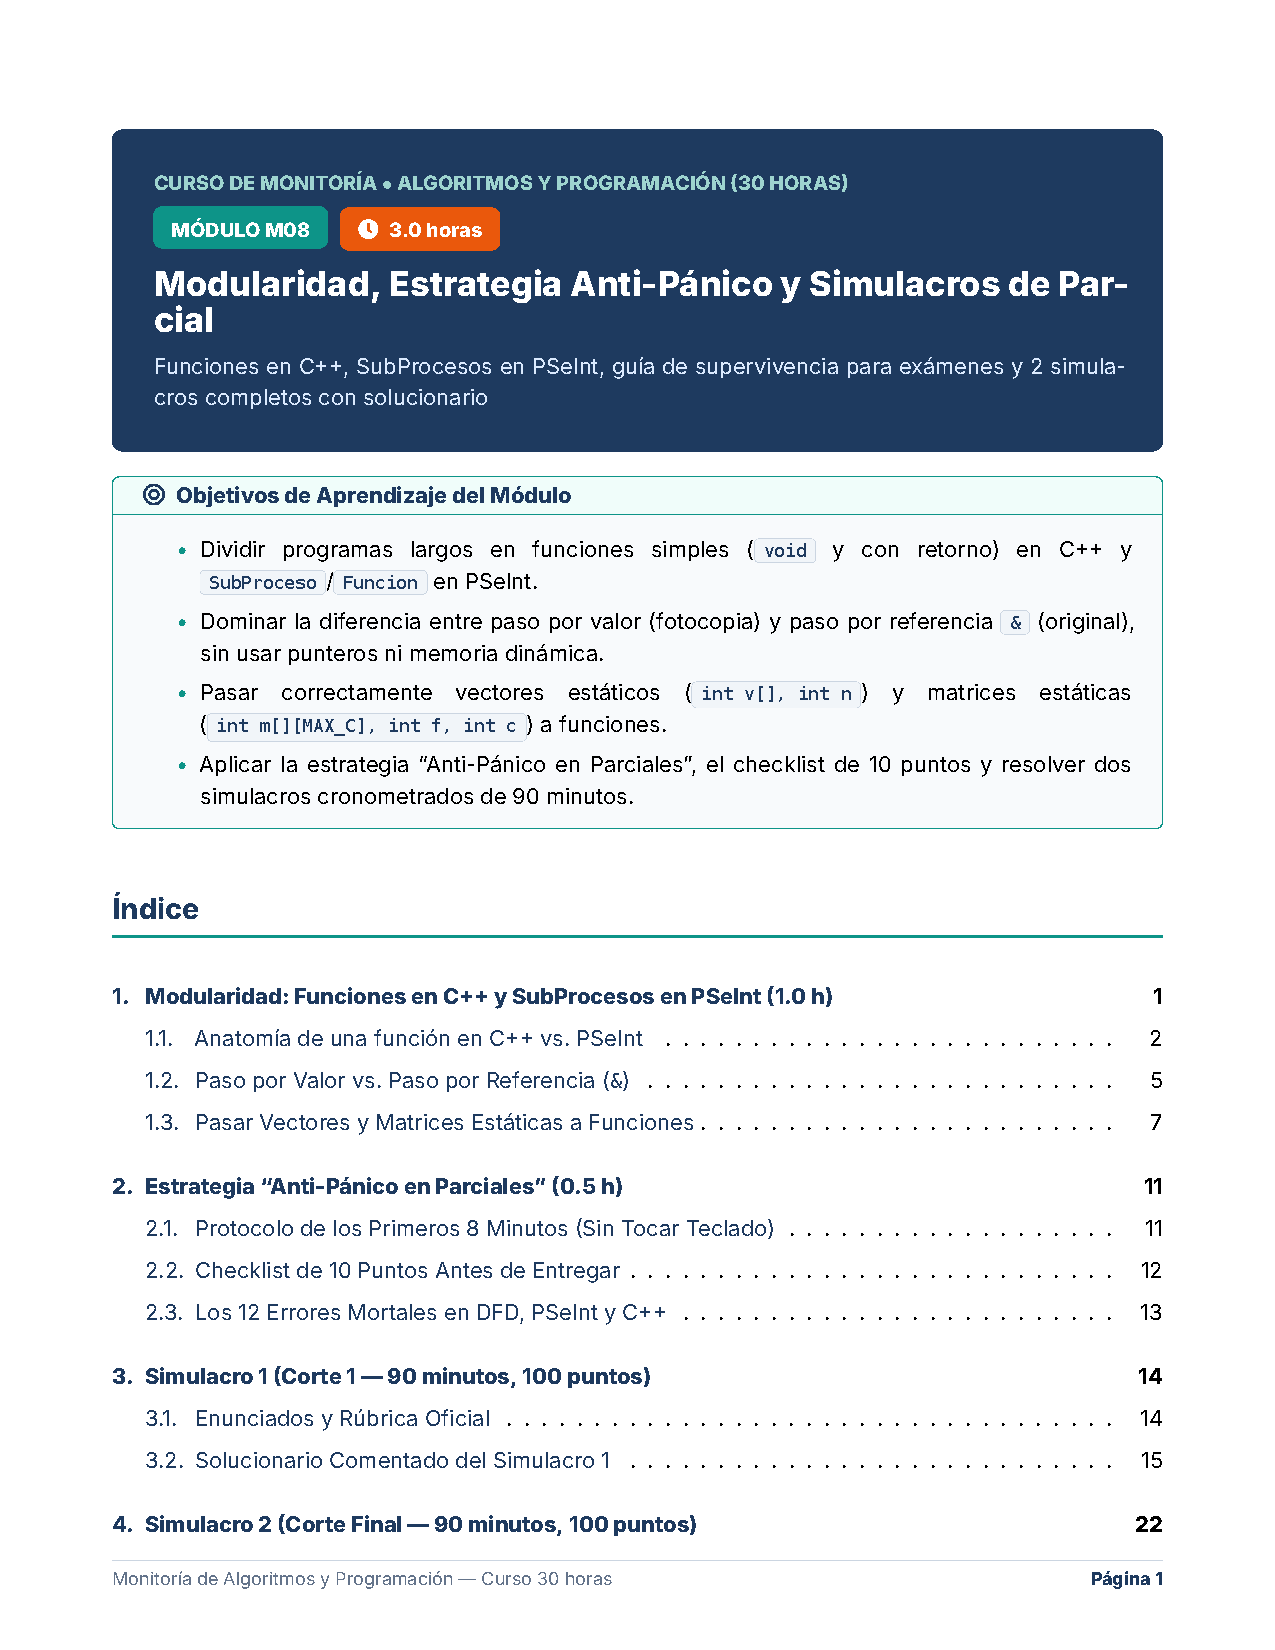
\includepdf[pages=-,addtotoc={1,section,1,{Módulo 08: Modularidad, Estrategia Anti-Pánico y Simulacros (3.0 h)},m08}]{modulos/M08_Modularidad_Parciales_y_Solucionario/M08_Modularidad_Parciales_y_Solucionario.pdf}

% ============================================================================
% APENDICE: 4 FICHAS RESUMEN IMPRIMIBLES
% ============================================================================
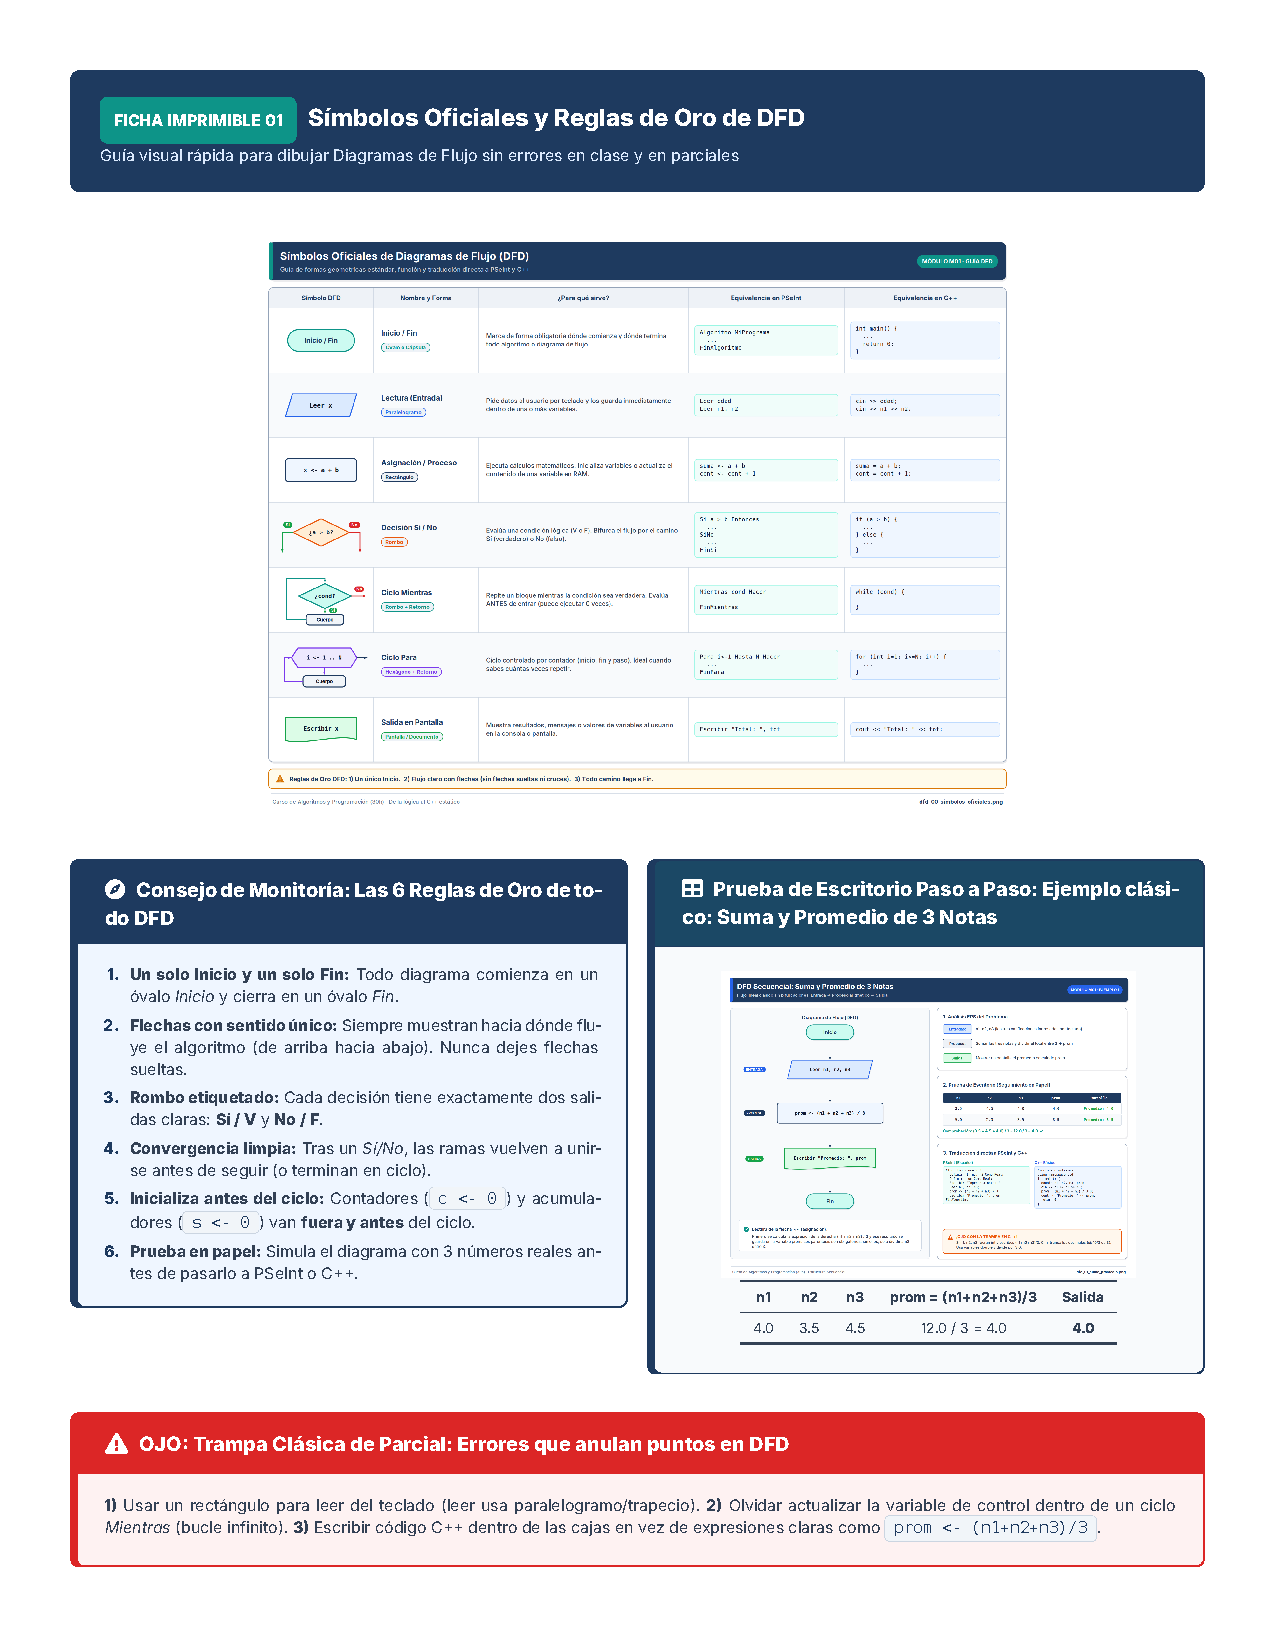
\includepdf[pages=-,addtotoc={1,section,1,{Ficha 01: Símbolos y Reglas de DFD},f01}]{fichas_resumen/Ficha_01_Simbolos_DFD.pdf}
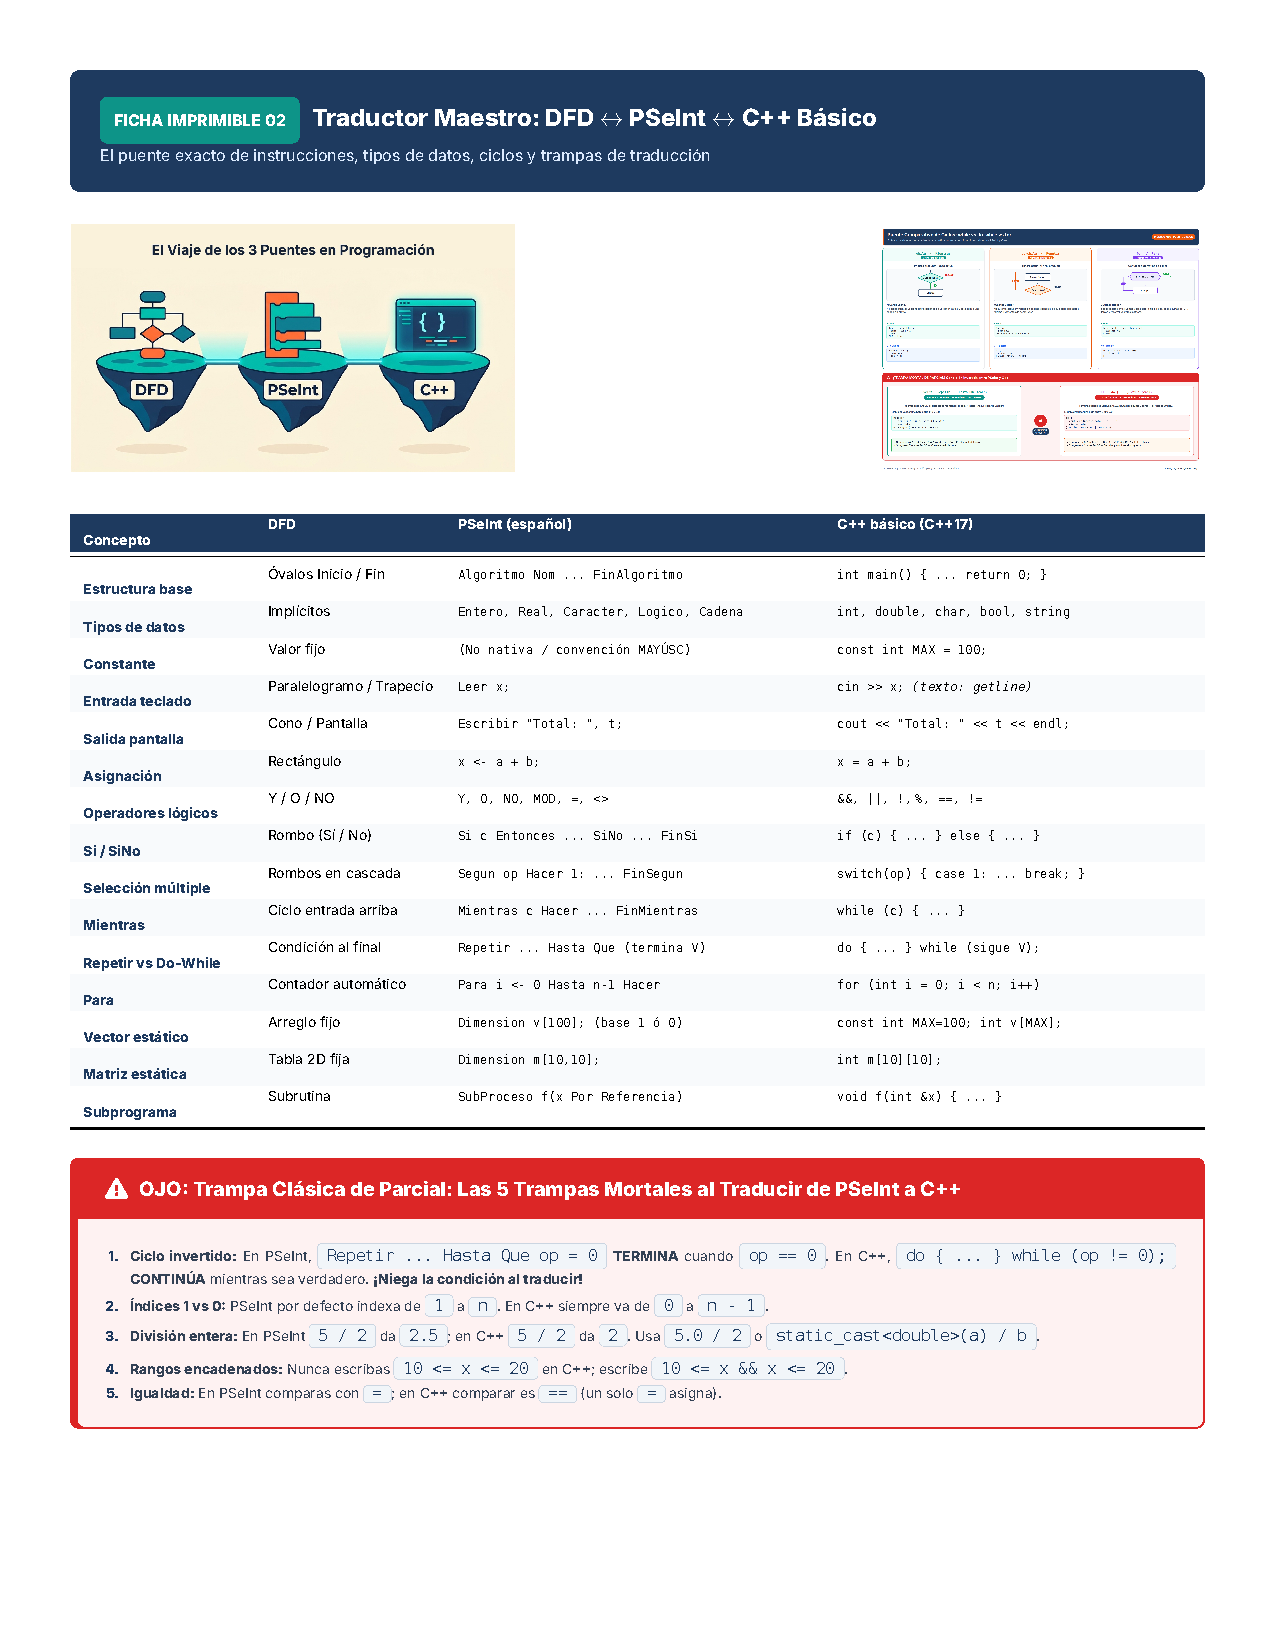
\includepdf[pages=-,addtotoc={1,section,1,{Ficha 02: Traductor DFD - PSeInt - C++},f02}]{fichas_resumen/Ficha_02_Traductor_DFD_PSeInt_CPP.pdf}
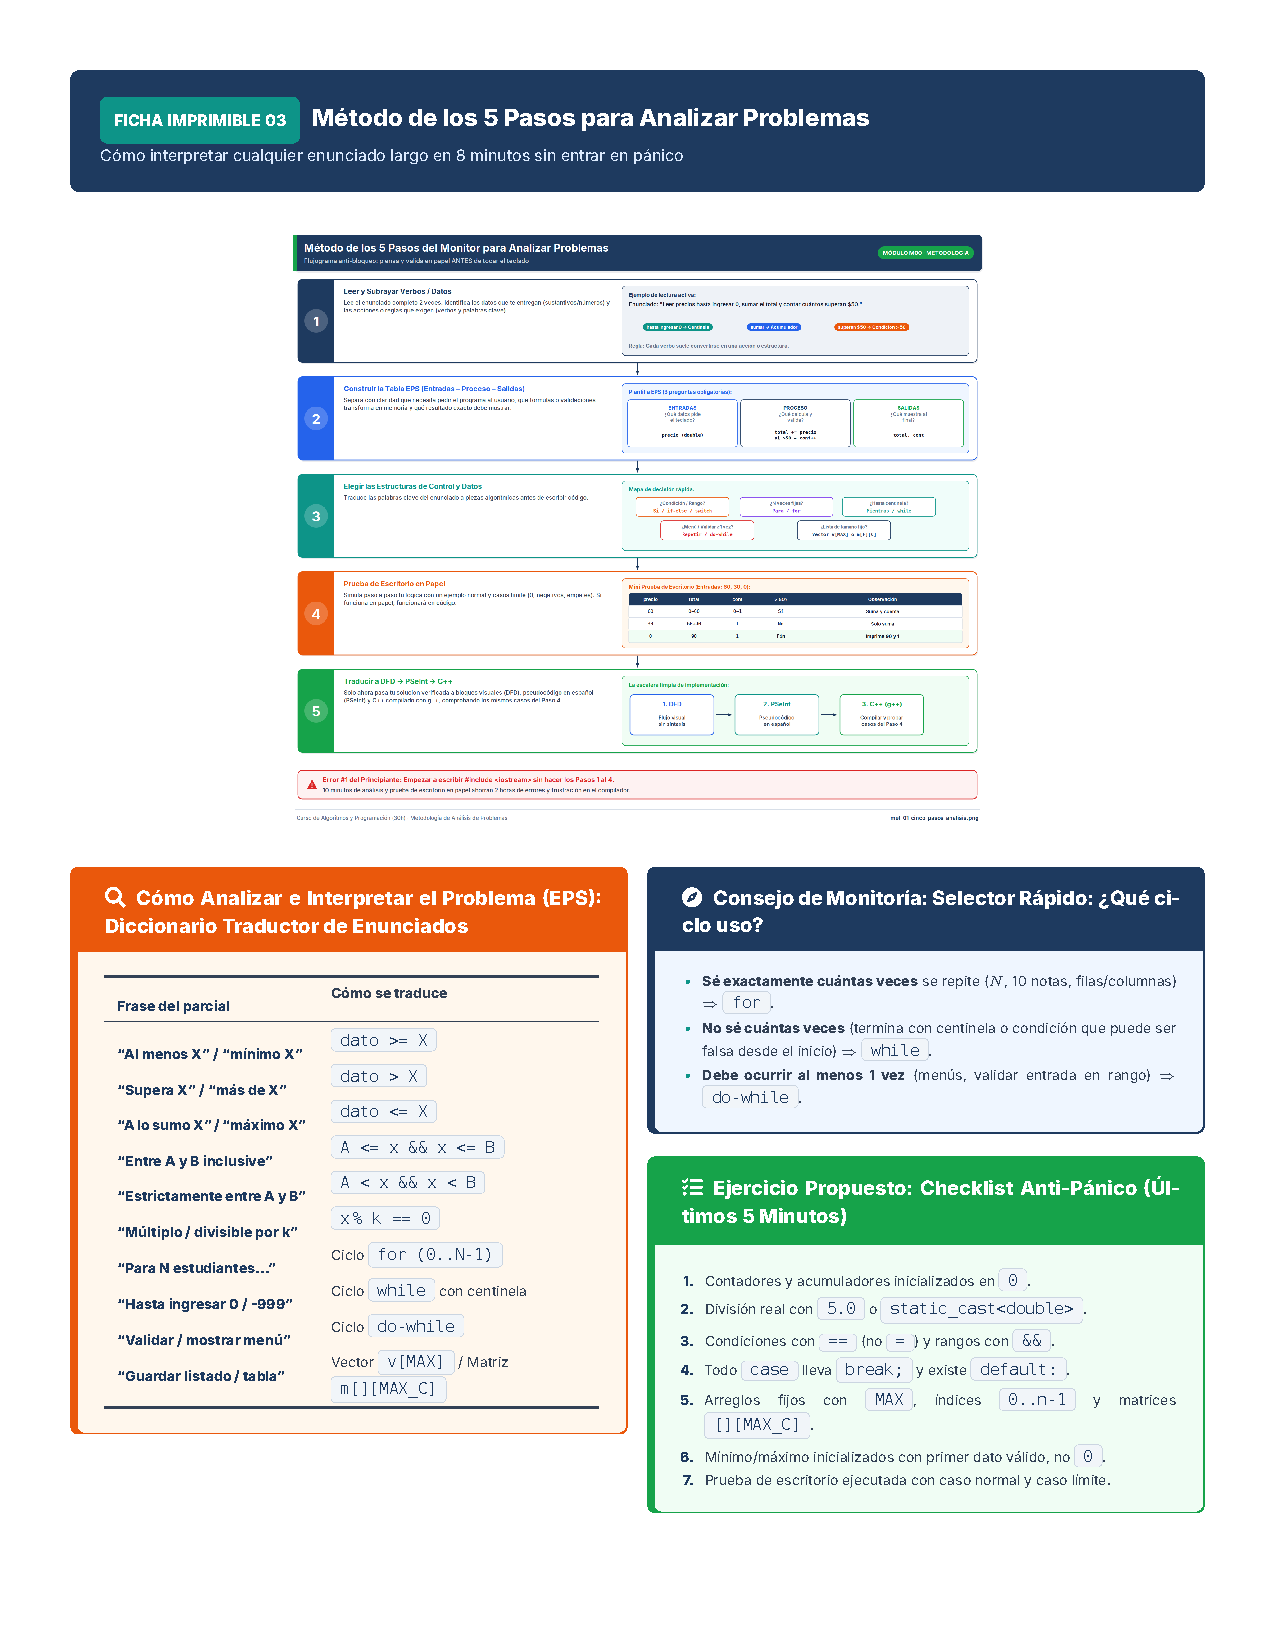
\includepdf[pages=-,addtotoc={1,section,1,{Ficha 03: Método de los 5 Pasos y Anti-Pánico},f03}]{fichas_resumen/Ficha_03_Metodo_5_Pasos_Analizar_Problemas.pdf}
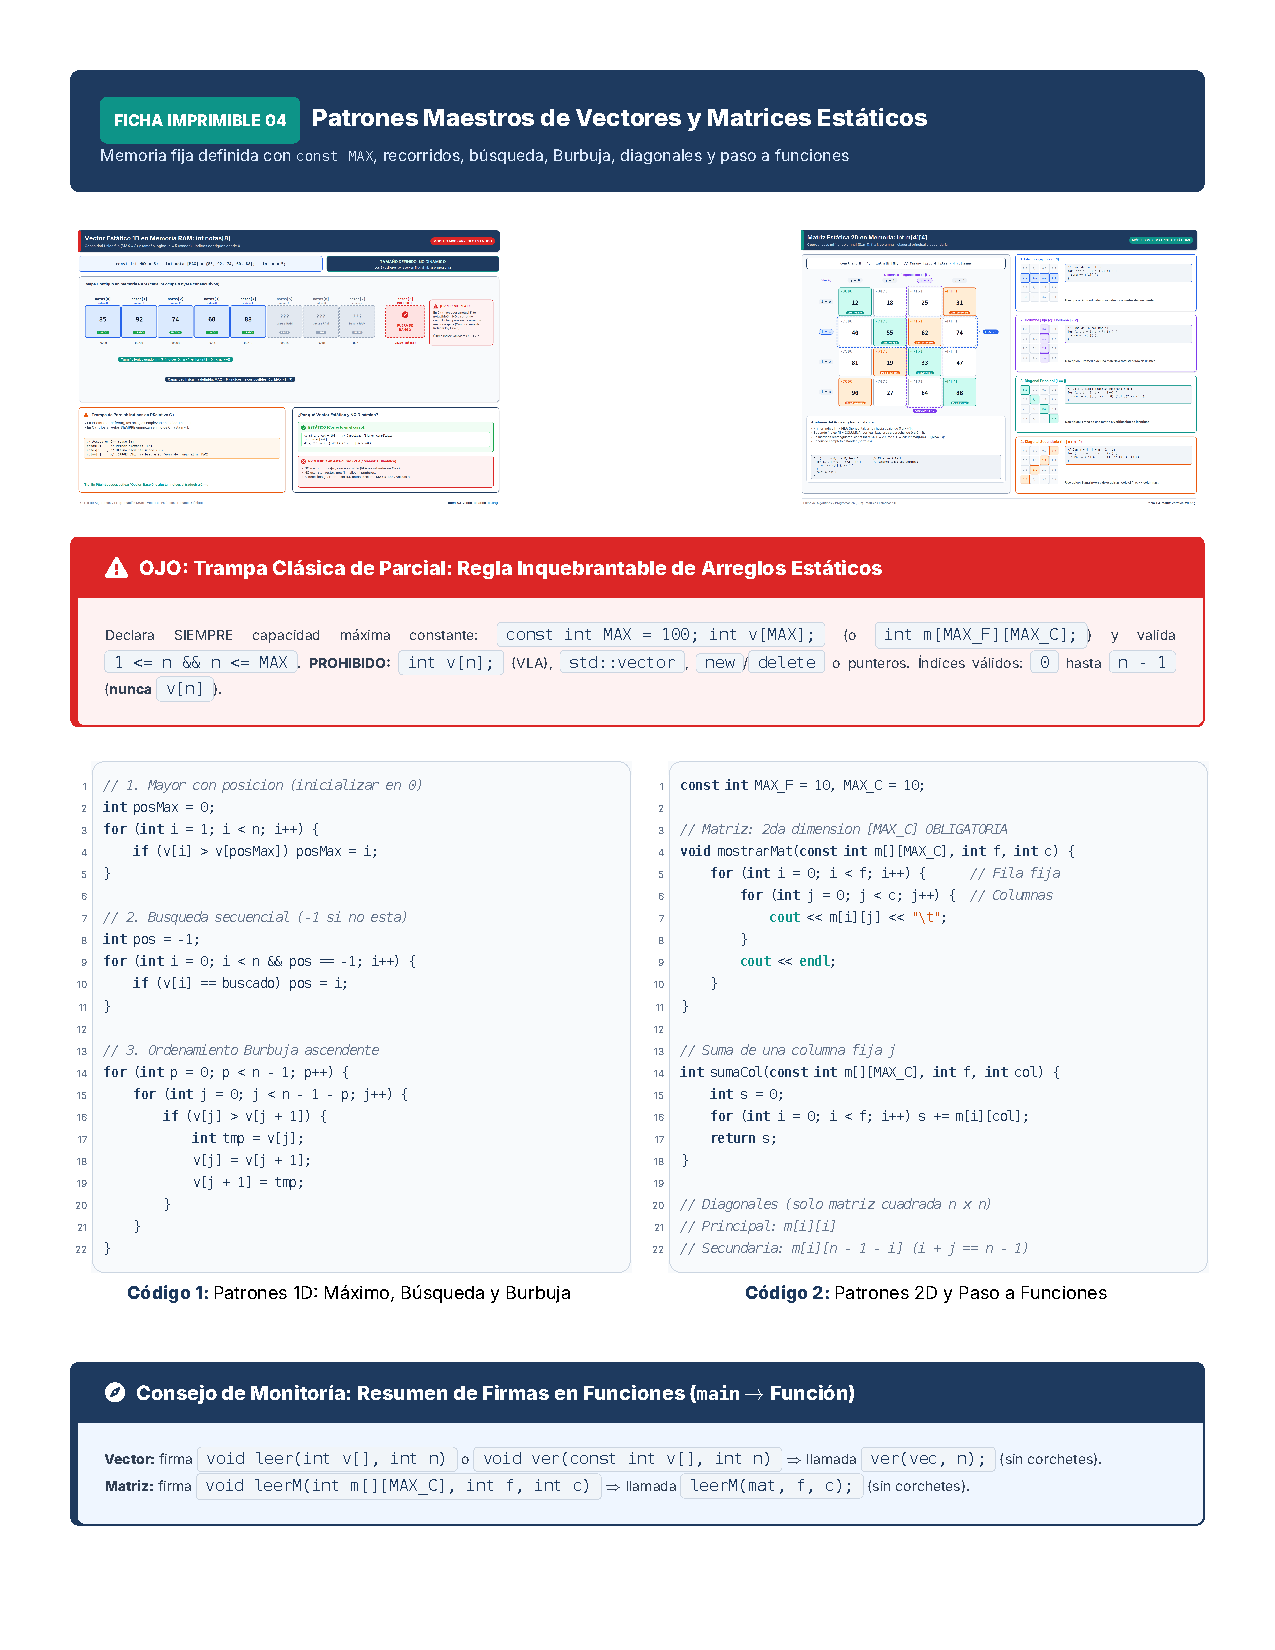
\includepdf[pages=-,addtotoc={1,section,1,{Ficha 04: Patrones de Vectores y Matrices Estáticos},f04}]{fichas_resumen/Ficha_04_Patrones_Vectores_y_Matrices_Estaticos.pdf}

\end{document}
